\documentclass[a4paper]{ctexart}
	\usepackage{geometry}
	\usepackage{enumerate}
	\usepackage{ntheorem}
	\usepackage{tikz}
	\usepackage[fleqn]{amsmath}
	\geometry{left=3.18cm,right=3.18cm,top=2.44cm,bottom=2.44cm}
	\title{A - Problem 300 in TCO Round 2A(Changed Version)}
	\author{何柱}
	\allowdisplaybreaks
\begin{document}
	\maketitle
	把$f(1)+f(2)+\ldots+f(R)$记成区间$[1,R]$,因为$f(0)=0$,不妨把区间变为$[0,R]$。如果没有$mod$,区间$[0,R]$的答案为$\frac{R(R+1)}{2}$。每次$mod$可以看成对区间进行切割,比如第一次$mod_1$把区间$[0,R]$切成$$[0,mod_1-1]*\lfloor\frac{R}{mod_1}\rfloor+[0,R \bmod mod_1]$$变成了至多两种类型的区间,其中一种区间只与$mod$的值有关,所以再次切割时又切成了至多三种类型的区间。经过$m$次切割后,原区间变成了至多$m+1$种类型的区间。设第$i$种区间为$[0,R_i]$,数量为$c_i$,则答案为$$\sum_{i=1}^{m+1}\frac{R_i(R_i+1)}{2}*c_i$$
	\begin{figure}[h]
		\begin{center}
			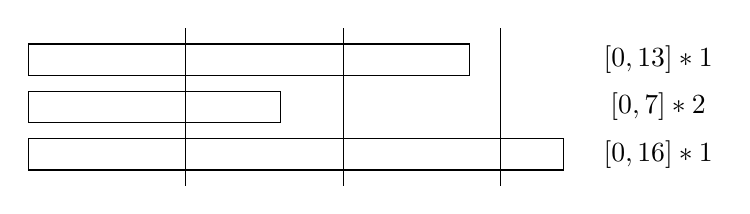
\begin{tikzpicture}[y=-1cm]
				\draw (0, 0.2) rectangle (5.6, 0.6);
				\node at (8.0, 0.4) {$[0, 13]*1$};
				\draw (0, 0.8) rectangle (3.2, 1.2);
				\node at (8.0, 1.0) {$[0, 7]*2$};
				\draw (0, 1.4) rectangle (6.8, 1.8);
				\node at (8.0, 1.6) {$[0, 16]*1$};
				\draw (2.0, 0.0) -- (2.0, 2.0);
				\draw (4.0, 0.0) -- (4.0, 2.0);
				\draw (6.0, 0.0) -- (6.0, 2.0);
			\end{tikzpicture}

			
\begin{tikzpicture}[y=-1cm]
			\draw[->,line width=2pt] (0.0, 0.0) -- (0.0, 0.6);
			\end{tikzpicture}

			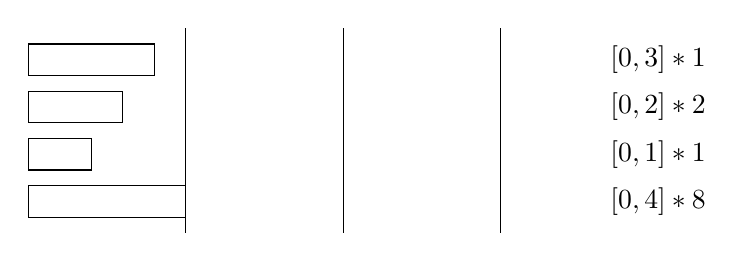
\begin{tikzpicture}[y=-1cm]
				\draw (0, 0.2) rectangle (1.6, 0.6);
				\node at (8.0, 0.4) {$[0, 3]*1$};
				\draw (0, 0.8) rectangle (1.2, 1.2);
				\node at (8.0, 1.0) {$[0, 2]*2$};
				\draw (0, 1.4) rectangle (0.8, 1.8);
				\node at (8.0, 1.6) {$[0, 1]*1$};
				\draw (0, 2.0) rectangle (2.0, 2.4);
				\node at (8.0, 2.2) {$[0, 4]*8$};
				\draw (2.0, 0.0) -- (2.0, 2.6);
				\draw (4.0, 0.0) -- (4.0, 2.6);
				\draw (6.0, 0.0) -- (6.0, 2.6);
			\end{tikzpicture}
		\end{center}
		\caption{将区间$[0, 13]*1$,$[0, 7]*2$,$[0, 16]*1$用$mod_i=5$切割的结果}
	\end{figure}
\end{document}